\section{Experiments with physical apparatus}
\label{s:exps}
The experiments with the inverted pendulum are run on the physical apparatus. The Figure \ref{fig:exps:componentsrollout} shows the components involved in making the new rollout. The new frame depicting the physical pendulum arrives at the local PC every $33$ ms. The state of the pendulum is then extracted from the frame. Basing on the state, the controller chooses the action to be applied. These two operations made by the local PC take negligible amount of time. Next, the action chosen by the controller is applied to the physical apparatus. The real state at time $t$ is used to apply the action at time $t+\Delta t$. The time delay $\Delta t$ is a result of capturing the state of the pendulum on the frame by the camera, sending the frame over to the computer and applying the new action. Before the new action $u_{t}$ is applied to the pendulum, the old action $u_{t-1}$ keeps being applied.

\begin{figure}[H]
\centering
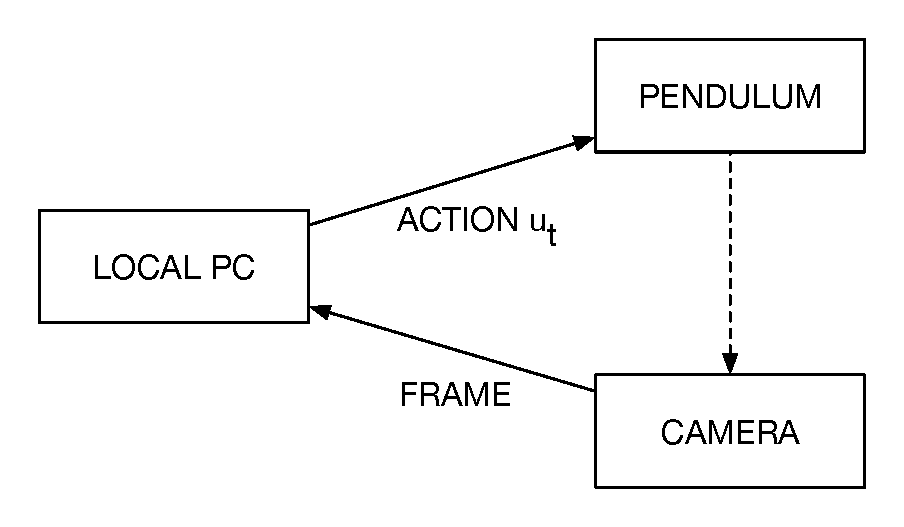
\includegraphics[width=0.5\textwidth, scale=0.5]{plots/rollout_components}
\caption{\label{fig:exps:componentsrollout} The components involved in the rollout of the physical pendulum. }
\end{figure}

\noindent Playstation 3 Eye is a cheap web camera used in this dissertation. It captures $30$ frames per second with the spatial resolution of $640x480$. Ignoring aberration effects, the move of the cart by one pixel in frame corresponds to $2$ mm distance move in the scenery. The Figures \ref{fig:exps:frame_single} and \ref{fig:exps:frame_double} show the example frames for single and double pendulum. The coloured blobs are attached to the cart and the ends of the pendulums. A color tracking algorithm is used to detect those points: a frame is converted into HSV\ (hue-saturation-value) color space and the pixels are masked, so only the pixels of the specific color\ (i.e. orange) are left. Then, the first moment of the locations of those pixels is calculated. Effectively, we calculate the center of the coloured blob. Indeed, the first moments marked as crosses, are at the centers of the coloured blobs on the Figures \ref{fig:exps:frame_single} and \ref{fig:exps:frame_double}. It is worth mentioning that the used color tracking algorithm is not lighting invariant (e.g., sunshine through the windows would affect its results).

\begin{figure}[!ht]
    \centering
    \begin{floatrow}
    \ffigbox[\FBwidth][\FBheight][t]{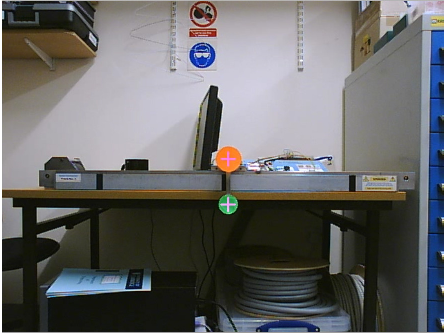
\includegraphics[width=60mm,scale=1]{plots/frame_single}}{\caption{The example frame with the single pendulum.}\label{fig:exps:frame_single}}
    \ffigbox[\FBwidth][\FBheight][t]{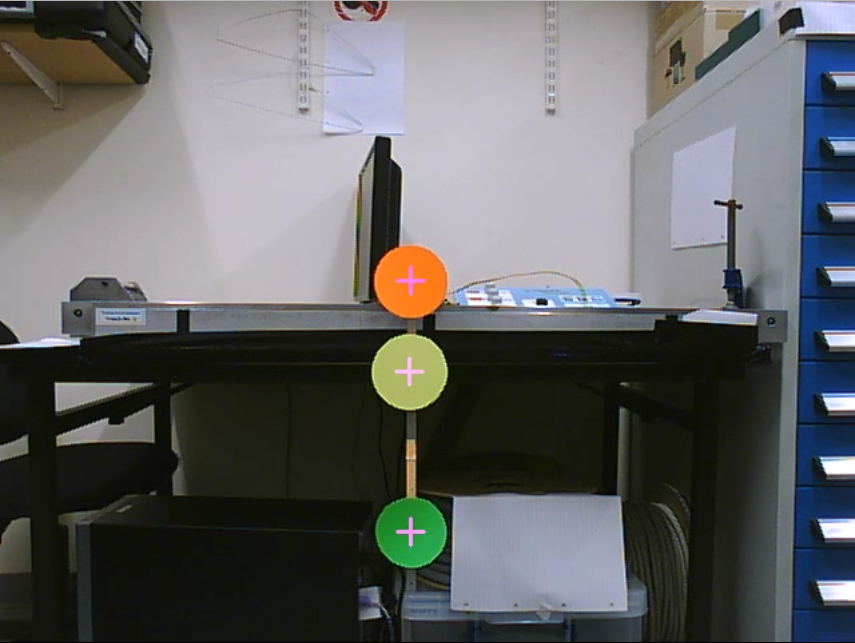
\includegraphics[width=60mm,scale=1]{plots/frame_double}}{\caption{The example frame with the double pendulum.}\label{fig:exps:frame_double}}
    \end{floatrow}
\end{figure}

\noindent For the running time speed, the program for making the rollouts is written in C/C++. It uses OpenCV library for communicating with the camera. The rollout data is sent from the local PC to the remote PC, which has 6 CPU cores. Next, the remote PC runs the PILCO framework written in MATLAB to learn the dynamics and policy models. Finally, the trained controller is sent back to the local PC and can be used for making the consecutive rollout.

\subsection{State representation}
\label{s:exps:state}
The color tracking algorithm presented in the previous section returns the current position of the cart $x$, as well as the ends of the pendulums. Those coordinates can be used to calculate the angles of the pendulums i.e. $\theta$ for the single pendulum problem. The full representation of the dynamical system also requires the cart velocity and the angular velocities of the pendulums. The velocities can be directly approximated from the previous and current values of $x$ and $\theta_{1}$. We know that the time difference between two consecutive frames is $dt=33ms$. The cart velocity can be approximated as $\dot{x}=\frac{x-ox}{dt}$, where $ox$ stands for the cart position from the previous frame. The full state representation for the single pendulum problem would be then:
\begin{equation}
[ou, x, \theta, \dot{x}, \dot{\theta}, u] \nonumber
\end{equation}
where $ou$ is the previous action applied to the system. As explained earlier, the action $u$ is applied with the time delay, and thus, the previous action $ou$ is also needed for the full representation of the state. 

\begin{figure}[H]
\centering
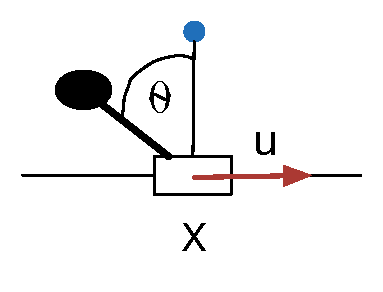
\includegraphics[width=0.5\textwidth, scale=0.5]{plots/pendulum_maths}
\caption{\label{fig:exps:statepend} The pendulum with the marked variables of the state.}
\end{figure}

\noindent The dynamics model for the above representation needs to predict 4 variables: $[x, \theta, \dot{x}, \dot{\theta}, u]$. Effectively, in PILCO, there will be a separate GP model for each variable. Each model will have its own noise level for the predicted variable. However, we know that there are only two noise sources per frame: noises on current cart position and the current end of the pendulum. PILCO would assume more noise sources than there, actually, are in the system.

\noindent The full state of the dynamical system can be also described by second order Markov representation. Instead of
approximating velocities, we can pass the previous and current $x$ and $\theta$ variables directly to the dynamics model. The belief is that the GP model itself will learn how to model the velocities out of those variables. Effectively, the state representation for the single pendulum would be then:
\begin{equation}
[oou, ox, o\theta, ou, x, \theta, u] \nonumber
\end{equation}
where $oou$ stands for the action applied before the previous frame; $ox$ and $o \theta$ are, respectively, a cart position and a pendulum angle extracted from the previous frame. 

\noindent The dynamics model for the second order Markov representation will try to predict only two variables: $x$ and $\theta$, since the rest of the new state representation can be copied over from the previous state. In PILCO, the dynamics model will consist of two GP models. This means that the dynamics will assume two sources of noise, which matches the amount of noise levels in the real system. Fewer GP models also shortens the training time of the PILCO framework.

\subsection{Delay and noise levels}
\label{s:exps:delaynoise}
The dynamics model does not need to know what the time delay is in the system. It can abstract over this parameter as long as the state of the dynamical system is fully represented. Full representation means that having the current state of the system, the next state of the system can be calculated in deterministic way. It is worth thinking how the full representation of the system would depend on different time delays. Frames from the camera come at the constant interval of $33$ ms and the delayed actions are believed to be also applied at the same constant interval. On the Figure\ref{fig:exps:camdelay}, the frames and the delayed actions are represented as $f_{t}$ and $a_{t}$, respectively, on the time axis. In this pictorial scenario, to calculate the frame $f_{t+1}$, we need two previous frames\ (i.e. second order Markov representation) along with all the actions, which affect those frames\ (including the calculated frame $f_{t+1}$). This mean that for calculating $f_{t+1}$, we need the following input: $[a_{t-2}, f_{t-1}, a_{t-1}, f_{t}, a_{t}]$. This is equivalent to the full representation of the inverted pendulum presented in the previous section. 

\begin{figure}[H]
\centering
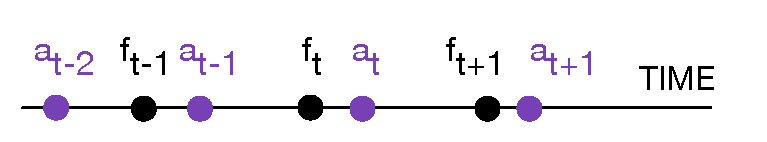
\includegraphics[width=0.5\textwidth, scale=0.5]{plots/cam_delay}
\caption{\label{fig:exps:camdelay} The frame $f_{t}$ and the delayed actions $a_{t}$ on the time axis. It presents the situation when the time delay is lower than the time between frames i.e. $33$ ms.}
\end{figure}

\noindent The time delay on the Figure \ref{fig:exps:camdelay} is represented as the time difference between applying the action $a_{t}$ and the frame $f_{t}$ itself. The higher time delay would mean that $a_{t}$ points are shifted in right direction. If the time delay is higher that the time difference between two consecutive frames, the $f_{t-1}$ frame would be affected by the action $a_{t-3}$. This changes the full representation of the system by adding older action $a_{t-3}$ to it. Thus, to determine whether the time delay in our experiments was higher than $33$ ms, the third order Markov representation\ (i.e. including action $a_{t-3}$) dynamics model was used. The linear component of the trained dynamics model had a very low value on the oldest action $a_{t-3}$. This was treated as an indicator that the dynamics can be successfully model without the additional action added. This effectively means, that the time delay is less than $33$ ms.

\noindent The locations of the coloured pixels are averaged to calculate the position of interests e.g., the cart position. The blobs themselves are the circles whose diameters equal to $20$ pixels. Each of those pixels represent the line along which the locations are averaged to get a horizontal position $x$ of the center of the coloured blob. Effectively, we have $20$ estimations of $x$ positions. For double inverted pendulum, the blobs were increased to the diameters of $49$ pixels to further reduce the noise level.

\subsection{Single pendulum}
\label{s:exps:single}
The experiments with the single physical pendulum of $12.5$ cm length were conducted. As mentioned earlier, the state of the system is described by the second order Markov representation:
\begin{equation}
[oou, ox, o \theta, ou, x, \theta, u] \nonumber
\end{equation}
There are $6$ state variables, where two of them\ (i.e. $x, \theta$) needs to be predicted by the dynamics model. As a policy model, the RBF network with $50$ radial basis functions is used. For PILCO dynamics model, there are $50$ pseudo points being used. For training the dynamics model as well as policy, $300$ iterations of BFGS algorithm is applied after each rollout. A single rollout lasts almost $2$ seconds, which corresponds to $60$ new samples for the dynamics model\ ($T=60$). The rollout can stop earlier if the cart hits one of the sides of the physical apparatus i.e. fail-safe mechanism\ (the pendulum track has the length of around $80$ cm: there is $40$ cm from the center to hit the side).

\noindent The trained dynamics model for this representation switched off the nonlinear GP model for cart position $x$by setting one of its length scale hyperparameters to very low value\ (i.e. $0.01$). At the same time, the linear part of the dynamics model behaves as expected: it models the next $x^{*}$ cart position by using previous and current cart positions, $ox$ and $x$:
\begin{equation}
x^{*} = 1.79 \times x - 0.79 \times ox = x + 0.79 \times (x-ox) \nonumber
\end{equation}
The next $x^{*}$ cart position is a current cart position plus its velocity. However, during the joint optimization of the linear and nonlinear model, this linear model is not known to the nonlinear GP model. At that time, the nonlinear GP thinks that it can not explain the data at all, and thus, it decides to switch itself off by setting very low length scale. The optimization procedure does not manage to switch the nonlinear GP on once the good linear model is achieved. This problem is mitigated if the linear components of the dynamics model are initialized more reasonable i.e. $2$ is a weight for $x$ and $-1$ for $ox$. Also, after rollout nr $13$, when there are $602$ training points for nonlinear GP, the $50$ pseudo points is not enough for modeling the dynamics. This is diagnosed by comparing the marginal likelihood of the full GP with sparse GP model as it was mentioned in the section \ref{s:pilco:ssm}. The amount of pseudo points is increased to $100$ from that rollout onward.

\noindent After $20$ rollouts and the total exposure of around $36$ seconds\ (i.e. $1074$ dynamics samples), the successful controller is learned by PILCO. Again, the dynamics's linear weights model the velocities:
\begin{equation}
\begin{split}
x^{*} = 1.76 \times x - 0.76 \times ox = x + 0.76 \times (x-ox) = x + 0.76 \times \dot{x} \\ \nonumber
\theta^{*} = 1.95 \times \theta - 0.95 \times o \theta = \theta + 0.95 \times (\theta-o \theta) = \theta + 0.95 \times  \dot{\theta} \nonumber
\end{split}
\end{equation}
The noise levels of the dynamics model are low. There is a $0.2^{\circ}$ observation noise on $\theta$. However, the observation noise is not propagated through the time-series model. All of the noise levels on $x$ are less than $0.025$ cm. 

\begin{figure}[!ht]
    \centering
    \begin{floatrow}
    \ffigbox[\FBwidth][\FBheight][t]{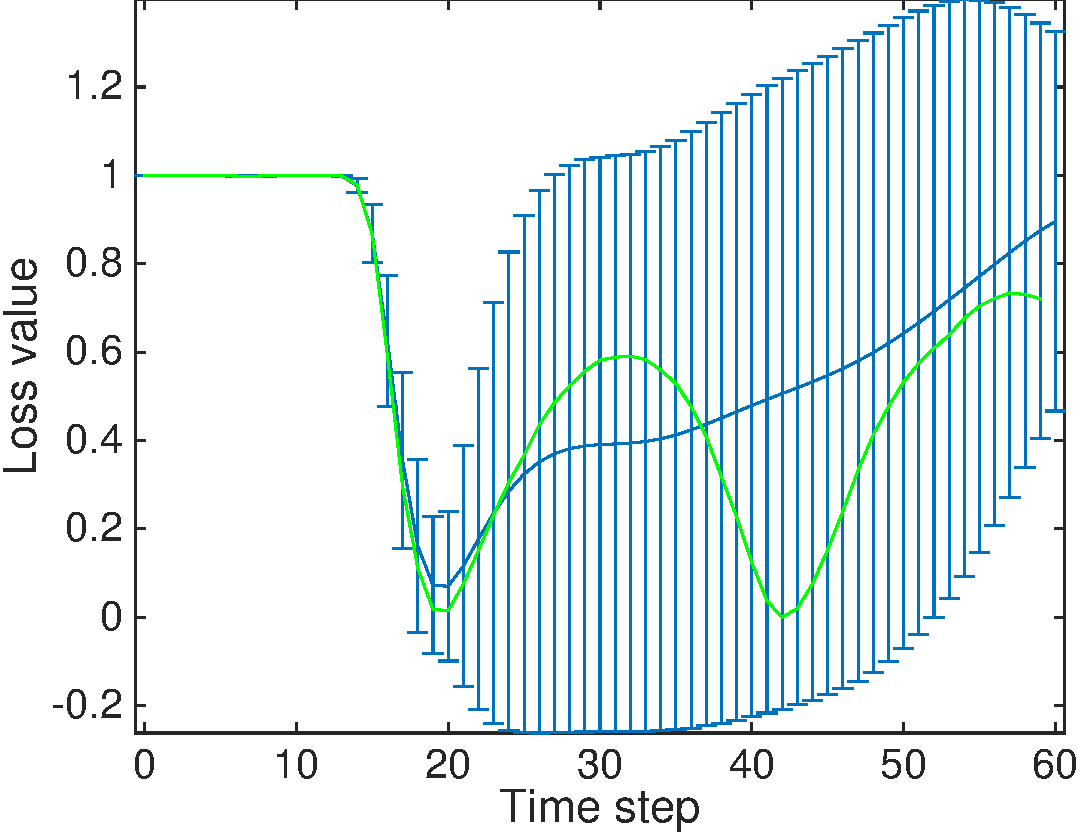
\includegraphics[width=60mm,scale=1]{plots/smk_loss}}{\caption{The predicted loss value of the trained controller for the single pendulum with the second order Markov representation. The green line corresponds to the rollout .}\label{fig:exps:single:2loss}}
    \ffigbox[\FBwidth][\FBheight][t]{\includegraphics[width=60mm,scale=1]{plots/smk_pred_x}}{\caption{The predicted trajectory of $x$. The blue error bars correpond to the variance multiplied by $2$.}\label{fig:exps:single:2predx}}
    \end{floatrow}
    \begin{floatrow}
    \ffigbox[\FBwidth][\FBheight][t]{\includegraphics[width=60mm,scale=1]{plots/smk_pred_theta}}{\caption{The predicted trajectory of $\theta$.}\label{fig:exps:single:2predtheta}}
    \ffigbox[\FBwidth][\FBheight][t]{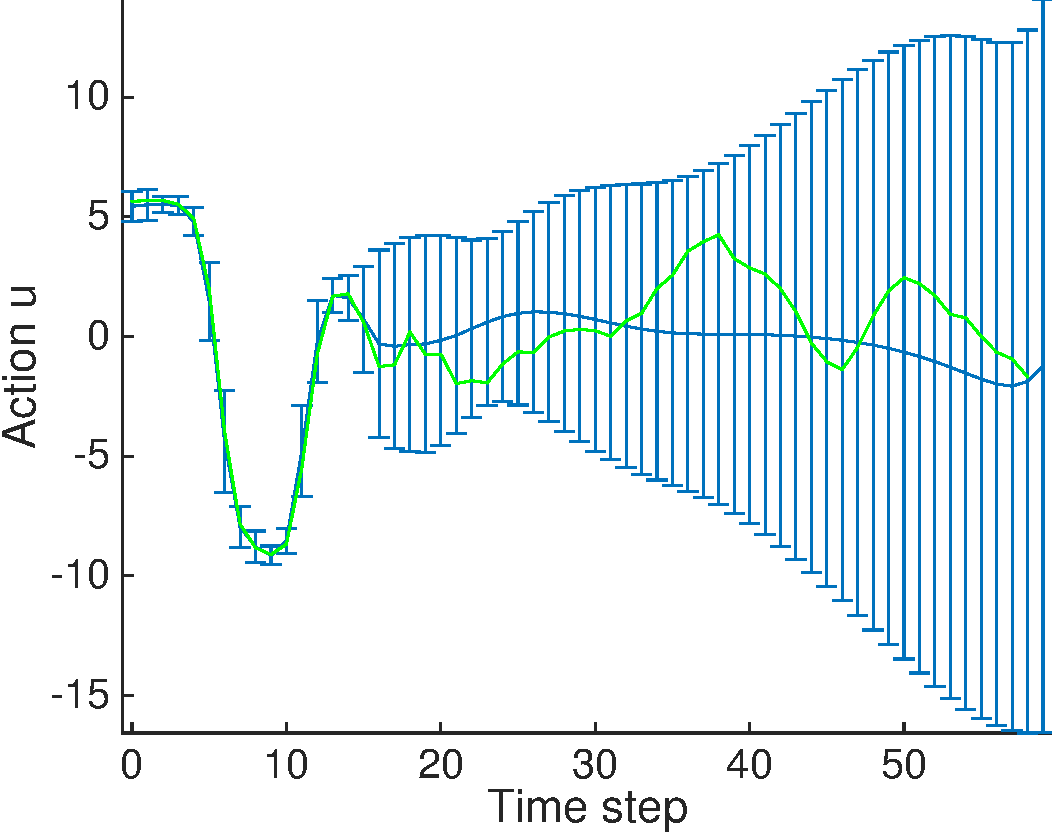
\includegraphics[width=60mm,scale=1]{plots/smk_pred_u}}{\caption{The predicted action applied to the pendulum.}\label{fig:exps:single:2predu}}
    \end{floatrow}
\end{figure}

\noindent The Figure \ref{fig:exps:single:2loss} shows the predicted loss value of the trained controller, where the Figures \ref{fig:exps:single:2predx}-\ref{fig:exps:single:2predu} show the predicted trajectory of $x$ and $\theta$ and the predicted action $u$ applied to the pendulum. First, the controller swings up the pendulum by applying positive action i.e. $5$ for few time steps, which is follow by maximum negative action i.e. $-10$. At that moment, the cart is heading towards its original position, but the pendulum is approaching the upright position\ (i.e. $\theta=0$). Then, the controller degrades its action to $0$, so the pendulum will actually slow down in the upright position and cart itself will stop around the origin.  Once this happens at $t=20$, the controller should start reacting depending on in which direction the pendulum wants to fall. At that time, the prediction on the state of the trajectory is not so tight anymore, since the controller is only reacting to the changes in the system. The prediction on trajectory matches the real rollout (i.e. green line), which means  the dynamics model is correct. More rollouts were made to determine the matching of the distribution to the samples.

\noindent Although the controller can keep the pendulum in the upright position, it does not guarantee to do it with the cart at the origin. To investigate it further, we linearize the policy at the target of the policy i.e. $ox=0, o\theta=0, x=0, \theta=0$: 
\begin{equation} \label{eq:exps:smk}
u=0.3007 + 0.07 \times (ox-0) + (-0.23) \times (\theta-0) \nonumber
\end{equation}
The weights of the $ox$ and $\theta$ seems small, which means that the controller is not so aggressive. This is likely to be because the variables are noisy. If the controller uses noisy variables to higher extent, it would inject further noise into the system making it more difficult to control. Tough, we have seen previously that the noise levels on the variables are relatively small according to our dynamics model. However, the noise could be also explained as the model uncertainty under the GP model. This would not be seen in the noise levels of our dynamics model.

\noindent Assuming that the dynamics model is correct, it seems that there are too much noise for the controller to do any better. As an experiment, the third order Markov representation is tried for modeling the dynamics. The bigger state representation should provide more information, which, possibly, should make the dynamics modeling easier. Indeed, the model with third Markov order representation yields better marginal likelihood for the same test dataset. Furthermore, the linear part of the GP models more complicated relationships between the variables:
\begin{equation}
\theta^{*} = 1.69 \times \theta - 0.43 \times o \theta -0.26 \times oo\theta + 1.07 \times x - 1.87 \times ox + 0.77 oox
\end{equation}
where $oo\theta$ and $oox$ stand for the angle and the cart position from the even older frame. New linear model for $\theta$ is interested not only in current angular velocity, but also in the previous one. Furthermore, $1.07 \times x - 1.87 \times ox + 0.77 oox$ is an acceleration filter on a cart position. For the same velocity of the cart $\dot{x}$, it will not have almost contribution  to the prediction of the next $\theta$. 

\noindent Another set of the experiments was run for the third order Markov representation. The new state of the system is:
\begin{equation}
[ooou, oox, oo\theta, oou, ox, o\theta, ou, x, \theta, u] \nonumber
\end{equation}
There were still two variables to predict i.e. $ou$ and $\theta$. The other settings of the experiments were the same as previously. During the training, there was no need to increase the amount of the pseudo points from $50$ to $100$. The successful controller was trained around iteration $14$, this kept training till the iteration $20$, so the total exposure time remains similar. 

\begin{figure}[!ht]
    \centering
    \begin{floatrow}
    \ffigbox[\FBwidth][\FBheight][t]{\includegraphics[width=60mm,scale=1]{plots/smk3_loss}}{\caption{The predicted loss value of the trained controller for the single pendulum with the thrid order Markov representation. The green line corresponds to the rollout .}\label{fig:exps:single:3loss}}
    \ffigbox[\FBwidth][\FBheight][t]{\includegraphics[width=60mm,scale=1]{plots/smk3_pred_x}}{\caption{The predicted trajectory of $x$.}\label{fig:exps:single:3predx}}
    \end{floatrow}
    \begin{floatrow}
    \ffigbox[\FBwidth][\FBheight][t]{\includegraphics[width=60mm,scale=1]{plots/smk3_pred_theta}}{\caption{The predicted trajectory of $\theta$.}\label{fig:exps:single:3predtheta}}
    \ffigbox[\FBwidth][\FBheight][t]{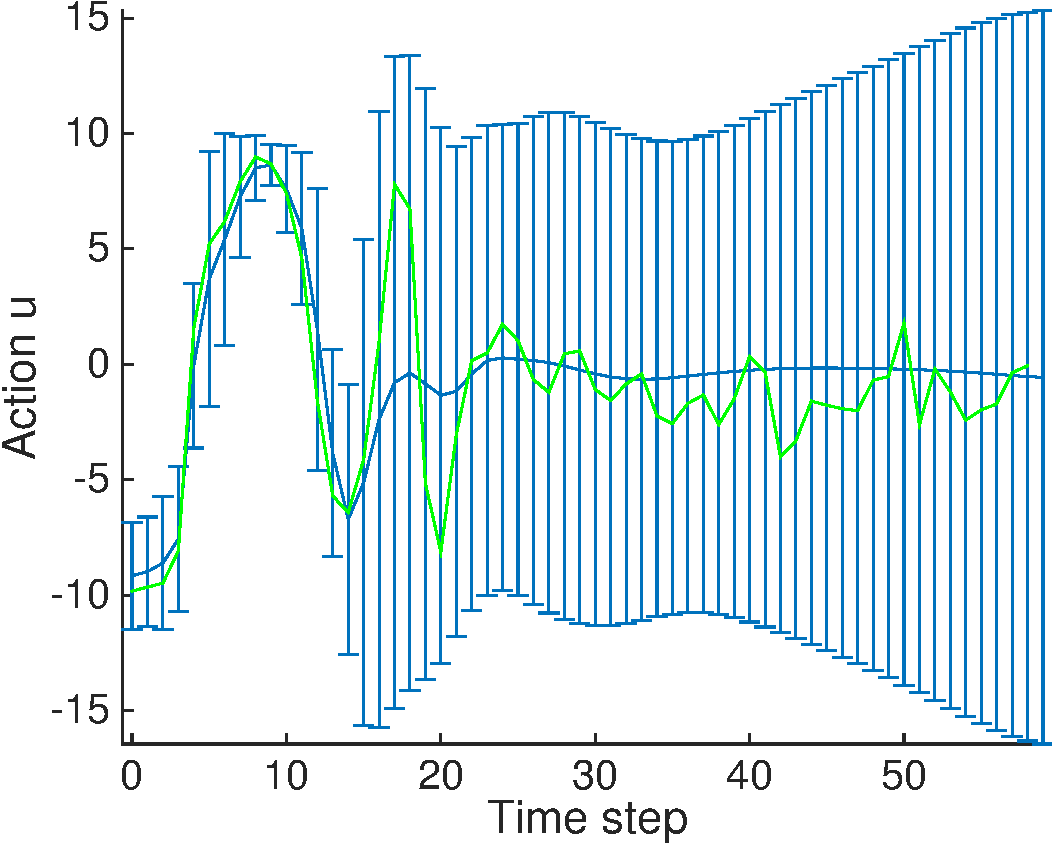
\includegraphics[width=60mm,scale=1]{plots/smk3_pred_u}}{\caption{The predicted action applied to the pendulum.}\label{fig:exps:single:3predu}}
    \end{floatrow}
\end{figure}

\noindent The Figure \ref{fig:exps:single:3loss} shows the predicted loss value of the new trained controller, where the Figures \ref{fig:exps:single:3predx}-\ref{fig:exps:single:3predu} show the predicted trajectory. In comparison to the trajectory shown on the Figures \ref{fig:exps:single:2predx}-\ref{fig:exps:single:2predu}, we can see that the state is better contained for later time steps i.e., lower error bar on the cart position and the angle. Similarly to the equation \ref{eq:exps:smk}, the controller is linearized at the upright position:
\begin{equation}
u=0.2831 + 1.08 \times (oox-0) + 1.08 \times (ox-0) + 1.08 \times (ox-0) + (-0.2) \times (\theta-0) \nonumber
\end{equation}
The new controller is more aggressive than the previous one. It assigns higher weights to the cart positions $oox, ox and x$. It also reacts depending on the current velocity of the cart, if there is any. Finally, it is also worth highlighting that the new controller swings the pendulum in other direction than the old one. This just experimentally shows that the original task is symmetric.

\subsection{Double pendulum}
\label{s:exps:double}
The experiments with the double pendulum were also run. In those experiments, the inner pendulum has a length of $12.5$ cm and the outer pendulum is longer, having the length of $22.7$ cm. We use the third order Markov representation for the state:
\begin{equation}
[ooou, oox, oo\theta_{1}, oo\theta_{2}, oou, ox, o\theta_{1}, o\theta_{2}, ou, x, \theta_{1}, \theta_{2}, u] \nonumber
\end{equation}
where $\theta_{1}$ represents the angle of the inner pendulum and $\theta_{2}$ of the outer one. The state has $12$ variables in total, where $3$ of those variables need to be predicted i.e. 3 separate GP models in our PILCO framework. Initially, $50$ pseudo points were used for the dynamics modeling. After the rollout nr $15$, the amount of the pseudo points was increased to $100$.

\noindent For the single pendulum, we specified the time horizon $T$ once and kept it the same through the whole task of learning. This does not seem enough to successfully learn the double inverted pendulum problem. The time horizon indirectly specifies what PILCO should learn. The Figure \ref{fig:exps:policytradeoff} compares the predicted loss of the two policies trained with different time horizon, but the same dynamics model. The blue error bars correspond to the policy with time horizon $T=40$, whereas the red blue bars represent the policy with $T=30$. The red policy performs better than the blue one with the exception of the last time step. The red controller swings up the pendulum faster, which allows it to achieve the upright position sooner and to have a tighter prediction on the state\ (time steps: 25-27). However, the upright state is lost immediately at time step 30, when the blue policy starts performing better. The blue policy trained on the longer time horizon prefers to swing up the pendulum slower, but then to have more chances to stabilize it in the upright position.

\begin{figure}[H]
\centering
\includegraphics[width=0.5\textwidth, scale=0.5]{plots/compare_pols}
\caption{\label{fig:exps:policytradeoff} The comparison of the predicted loss: the blue error bars represent the policy trained over the time horizon $T=40$, whereas the red error bars is the policy trained over $T=30$.}
\end{figure}

\noindent On the other hand, if the time horizon is too long, this has the implications for the dynamics model. There will be more samples for the dynamics model, but most of them will come from the regions of space, which are not crucial for successfully learning the whole task. In another series of the experiments, the time horizon was set to $60$. PILCO managed to learn how to swing up the first pendulum\ (time step $10-15$), but could not succeed on swinging up both pendulums\ (time step $15-25$). Then, instead of making further progress on it, PILCO started optimizing what actions to take when both pendulums are already dropped at time steps $40-50$. This may be also just an indicator that the dynamics model is not correct and the policy just adapts to this scenario. The longer rollouts also mean longer training time of the dynamics model. For our experiments with the double pendulum, we decided to start with time horizon $T=30$, and then, keep increasing it by another $5$ times steps if we think that we are dealing with the situation similar to the one from the previous paragraph.

\subsubsection{Sequence of linear models as policy representation}
\label{s:exps:double:policyrep}
The double inverted pendulum is more challenging problem, which requires more rollouts to learn the successful controller. After each rollout, the policy is being retrained from the previous optimal controller. One may be afraid whether the policy will not become too convoluted after many epochs of training. Indeed, it was noticed around the iteration nr $40$ that the policy learning did not continue to progress any more tough the dynamics model did. The mean cost of the predicted trajectory could be no further optimized. As mentioned earlier, the RBF network was used as a policy model. The Figure \ref{fig:exps:rbfactt} shows the mean output contributions of the individual units of the RBF network along the predicted trajectory. In optimization, some of those contributions need to change in order the controller to have the new predicted trajectory with lower mean cost. However, some of those contributions are not only high values, but they also cancel each other out. The Figure \ref{fig:exps:rbfcancel} shows how two high values contributions when added result in relatively small contribution function. Two units are highly coupled, the slight change in the position or height of one unit will result in significantly different function. This situation is not preferable for optimization, since it can not easily optimize any of those units. 

\begin{figure}[!ht]
    \centering
    \begin{floatrow}
    \ffigbox[\FBwidth][\FBheight][t]{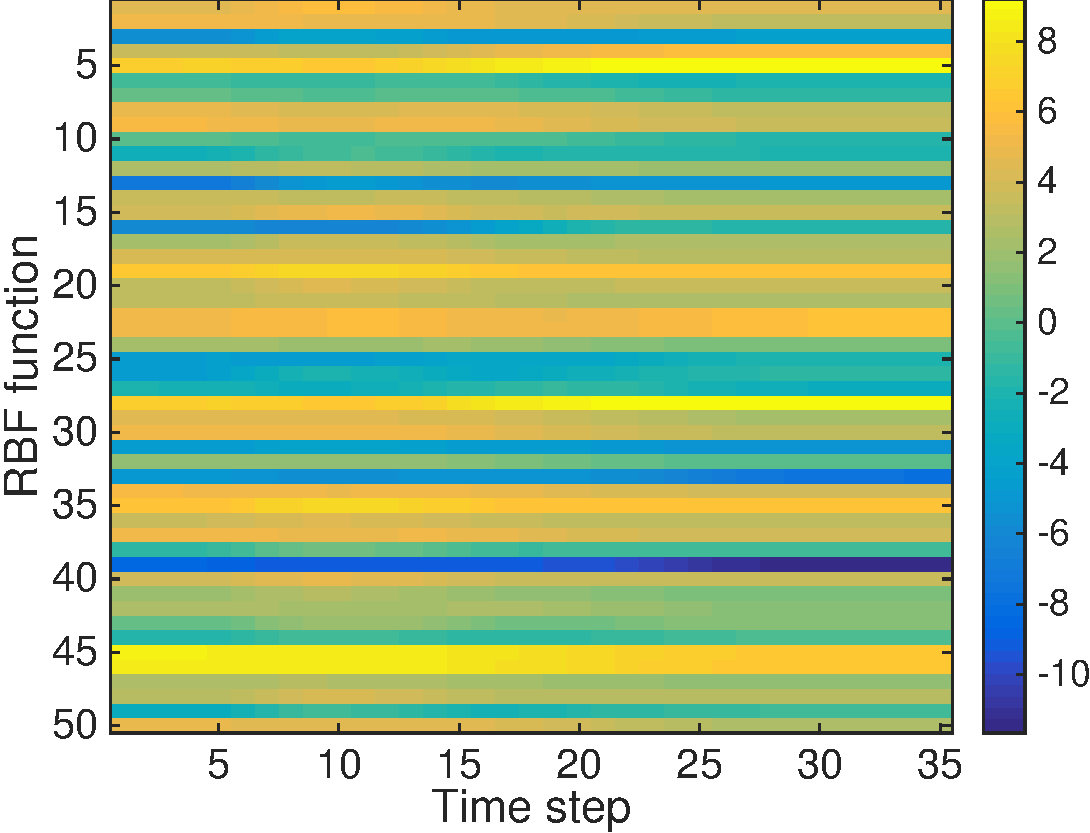
\includegraphics[width=60mm,scale=1]{plots/rbf_actt}}{\caption{The mean output contributions of the individual units of the RBF network along the predicted trajectory of the trained controller. The absolute values of those contributions are shown in the logarithm space (i.e. color value of $8$ corresponds to $29810$).}\label{fig:exps:rbfactt}}
    \ffigbox[\FBwidth][\FBheight][t]{\includegraphics[width=60mm,scale=1]{plots/rbf_cancel}}{\caption{The contribution for the predicted tracjectory of the unit $5$\ (blue line) and unit $28$\ (red line) of the RBF network. The contribution from both units cancel out when added\ (yellow line).}\label{fig:exps:rbfcancel}}
    \end{floatrow}
\end{figure}

\noindent To mitigate the above problem, the RBF policy has been converted to the sequence of linear models proposed in this dissertation \ref{s:pilco:seqlin}. The output distribution from the RBF policy is always approximated by moment matching. The linear output distribution is computed at each time step along the predicted trajectory to obtain the sequence of the linear models. This new policy will apply exactly the same actions as the RBF controller. However, the separate linear models do not infer over time, and thus, are unlikely to become highly coupled. This seems crucial for further successful learning that the controller can be optimized over many rollouts without getting convoluted.

\noindent Knowing that just one linear controller $\overline{\pi}$ can stabilize the double pendulum in the upright position, one may wonder how the sequence of the linear models will cope with the stabilization task itself. A successful sequence of linear models controller should simply duplicate $\overline{\pi}$ controller $T$ times. We believe that this will be indeed achieved in the training procedure. If the first controller $pi_{0}$ of the sequence is successfully learned and matches the $\overline{\pi}$ controller, then we can assume that the output state distribution after applying the action from that controller will be the same as the input distribution for that controller. That simply means that as a result of applying the new action, the state of the system did not change. With some simplification, we know that this should be true, since the controller aims to keep the pendulum in the upright position. If the one model of the sequence is successfully learned and the output state does not change, the next linear model of the sequence will be also learned since the same dynamics model is used. By induction, the whole sequence of the linear models will be successfully learned.

\subsubsection{Dynamics model}
\label{s:exps:double:dyns}
Around the rollout nr $50$, the sequence of the linear models arrived at the suboptimal parameters, which did not change over the next few rollouts. As we said in the previous section, the new policy model is very flexible to be optimized, since the separate linear models do not interfere over time. The policy training does not progress any further, since the dynamics model does not provide the policy with any new information. The dynamics model is either not good enough or there is simply too much noise in the system to successfully learn the task.  

\noindent The trained GP Time-Series model has $0.22^{\circ}$ process noise on the $theta_{1}$ prediction, which is propagated to the consecutive latent states of the time series model. It is not clear whether this process noise stops the policy from progressing. To address this issue, the experiment with learning only the subtask of the main task was proposed. The policy gives us the predicted trajectory of the state, which spans over the time horizon $T=40$. We can freeze our policy and dynamics model over first $20$ time steps and try to learn the new task from the time step $t=21$ onward. The separate dynamics model can be used only for this subtask. One can select the dynamics samples from each rollout just basing on time i.e. take the second half of each rollout\ (from $t=21$ onward). The dynamics model trained this way has the process noise on $theta_{1}$ close to $0$, instead the observation noise is close to  $0.22^{\circ}$. This is preferable behaviour of the model, since the observation noise is not going to be propagated through the time-series model. On the other hand, the dynamics model for the new subtask has a process noise of $0.13$ on $theta_{2}$. 

\noindent The policy was also trained for the new subtask using its new dynamics model. The policy performs better than the main policy from time step $t=21$ onward in the main task. The difference between two policies is even higher if the time boundary is chosen as $t=18$\ (the main policy has a tight prediction on the state at that time step). The Figure \ref{fig:exps:subtask:loss} compares the predicted loss of both controllers. The policy of the subtask has tighter predicition around the upright position\ (i.e. time steps $23-26$). On the Figure \ref{fig:exps:subtask:theta2}, we can also see how better the prediction on the $\theta_{2}$ angle is in the policy of the subtask in comparison to the old policy. With the new subtask controller, $20$ rollouts were conducted, which confirmed that the prediction on the trajectory matches the samples from the real system.

\begin{figure}[!ht]
    \centering
    \begin{floatrow}
    \ffigbox[\FBwidth][\FBheight][t]{\includegraphics[width=60mm,scale=1]{plots/compare_subtask_loss}}{\caption{The comparison of loss of the predicted trajectory from time step $t=18$. Blue error bars correspond to the main policy, while the green are the subtask's policy.}\label{fig:exps:subtask:loss}}
    \ffigbox[\FBwidth][\FBheight][t]{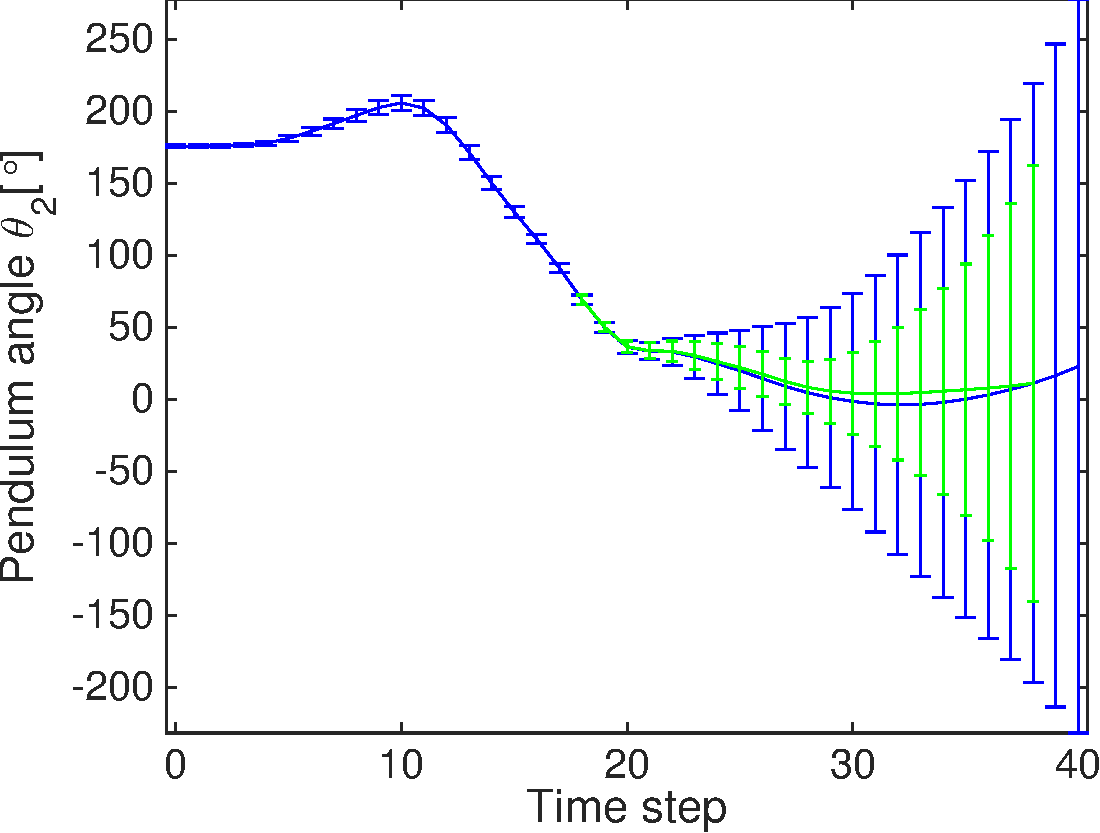
\includegraphics[width=60mm,scale=1]{plots/compare_subtask_theta2}}{\caption{The comparison of the predicted trajectory according to the main policy\ (blue) and subtask's one\ (green).}\label{fig:exps:subtask:theta2}}
    \end{floatrow}
\end{figure}

\noindent The results of the above experiment indicate that the previously trained dynamics model is not good enough. It is possible that one parametric GP model is not able to capture the whole dynamics of the system. The GP is used with squared exponential which is a stationary covariance function. The dynamics of the double pendulum may be non-stationary. The pendulum behaves differently when it is being swung up with high angular velocity and when it slows down around the upright position. This dynamical system can be also tackled by using more GPs in the time-series model as it is proposed in this dissertation\ (section \ref{s:pilco:ssm}). Effectively, the task can be split onto smaller subtasks, which can be learned in joint optimization.

\noindent If more GPs are plugged to the time-series model, the samples may be assigned to different GPs also  on state-based criterion. Instead of splitting the samples by time, we can filter the rollout which pass through the specific state distributions. For example, if we want to model the subtask of stabilizing the pendulum, we can filter only those parts of rollouts in which latent state or observation itself is in upright position. The dynamics models with such a state filtering have been also trained. Such a compound dynamics model yields slight improvement into the policy. Another extension to the Direct Method for GP Time-series model proposed in this dissertation\ (section \ref{s:pilco:ssm}) is training pseudo inputs. Although the method has worse time complexity, it was used to determine whether the time-series model with one GP would perform better. It turns out that the trained model with the movable pseudo inputs overfits the data by yielding unrealistic low noise levels. 

\noindent When modeling high dimensional problem, the FITC algorithm may tend to put the pseudo points on the sphere of the data points, instead of putting them next to the training points. This results in the higher variance in the regions of the training points. The marginal likelihood optimization should try to the pseudo points next to the training points, but this may not happen. This phenomenon could be a possible reason of the problems we encounter while using the GP tim-series dynamics model. In the time-series model, the locations of the pseudo points are pre-trained by FITC. The non time-series GP model, which does not account for the noise in the input was also trained on the whole accumulated data. This was followed by training new policy model, which seems promising. In simulations, the controller thinks that it can successfully control the double inverted pendulum. However, the samples from the real system do not match the predicted trajectories.

\subsubsection{Controller}
\label{s:exps:double:ctrl}
The predicted loss and the trajectory of the best trained controller are shown on the Figures \ref{fig:exps:double:3loss}-\ref{fig:exps:double:3predu}. The controller uses three separate dynamics model which are split by time: the first GP for time steps from $1$ to $18$, the second GP from $19$ to $25$ and the last GP from $26$ to $40$. All of the dynamics model are trained in joint optimization, as well as the main policy consisting of policies of the three subtasks.  The total exposure time was $112$ seconds, which corresponds to $3386$ training samples.

\noindent The controller first swings up the outer pendulum in the similar fashion to the controller in the single pendulum problem: by applying few times strong positive action followed by the series of strong negative actions. The swing up of the outer pendulum happens just before time step $t=20$. Then, the outer pendulum is pushed out, which is followed by the swinging up of the inner pendulum. As the result of the swinging up two pendulums, the pendulum are close to being  colinear. At time step $t=27$, the angle of the first pendulum first pendulum is $-10^{\circ}$, where the angle of the second pendulum is $10^{\circ}$. The mean predictions on those angles go steadily in opposite direction, which means that the pendulums are expected to become colinear. However, the prediction on the time step $t=30$ is not tight enough for the pendulums to be guaranteed to become colinear. Nevertheless, then, the pendulums tried to be stabilize. It happened once on twenty additional rollouts that the pendulums were actually stabailized till the end of the time horizon\ (this would not be a case if the time horizon was longer). Under the simulations, we have also observed that the algorithm tries to swing up both of the pendulums at the beginning at the same time. This is achieved by slowly swinging the pendulum in both directions. However, as a result, the pendulums are already colinear when they approach the upright position.

\begin{figure}[!ht]
    \centering
    \begin{floatrow}
    \ffigbox[\FBwidth][\FBheight][t]{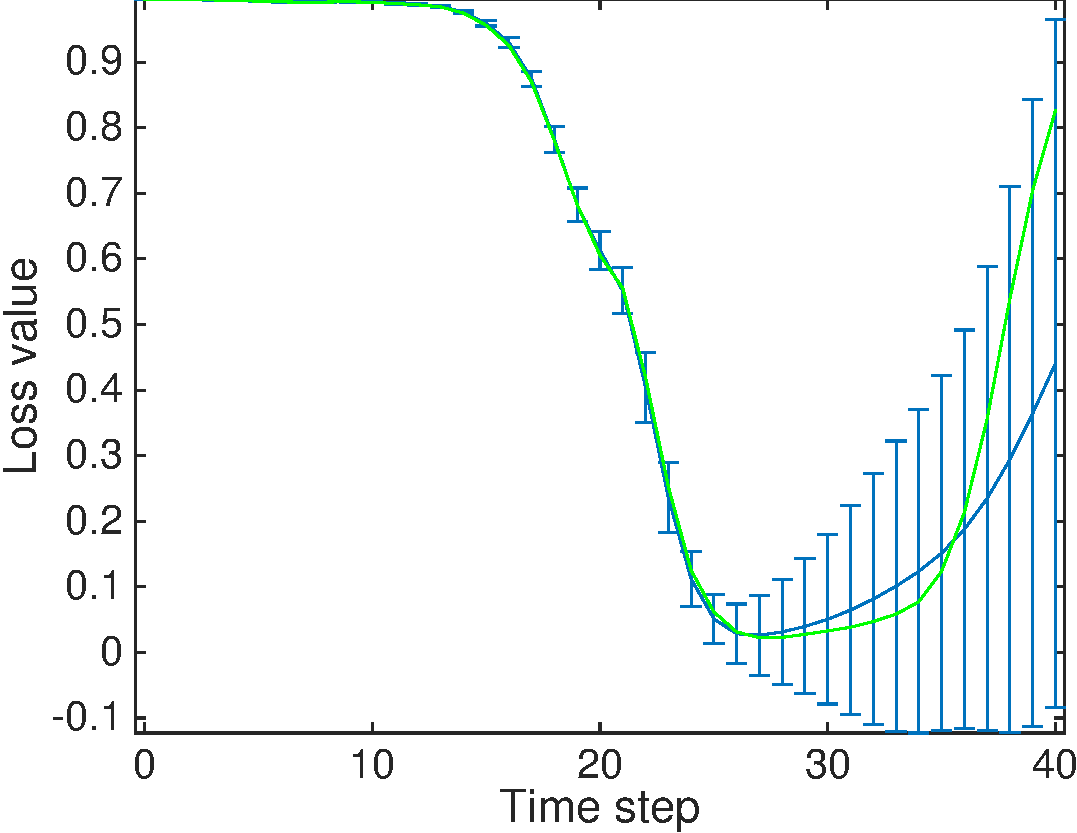
\includegraphics[width=60mm,scale=1]{plots/dmk3_loss}}{\caption{The predicted loss value of the trained controller for the double pendulum with the thrid order Markov representation. The green line corresponds to the rollout .}\label{fig:exps:double:3loss}}
    \ffigbox[\FBwidth][\FBheight][t]{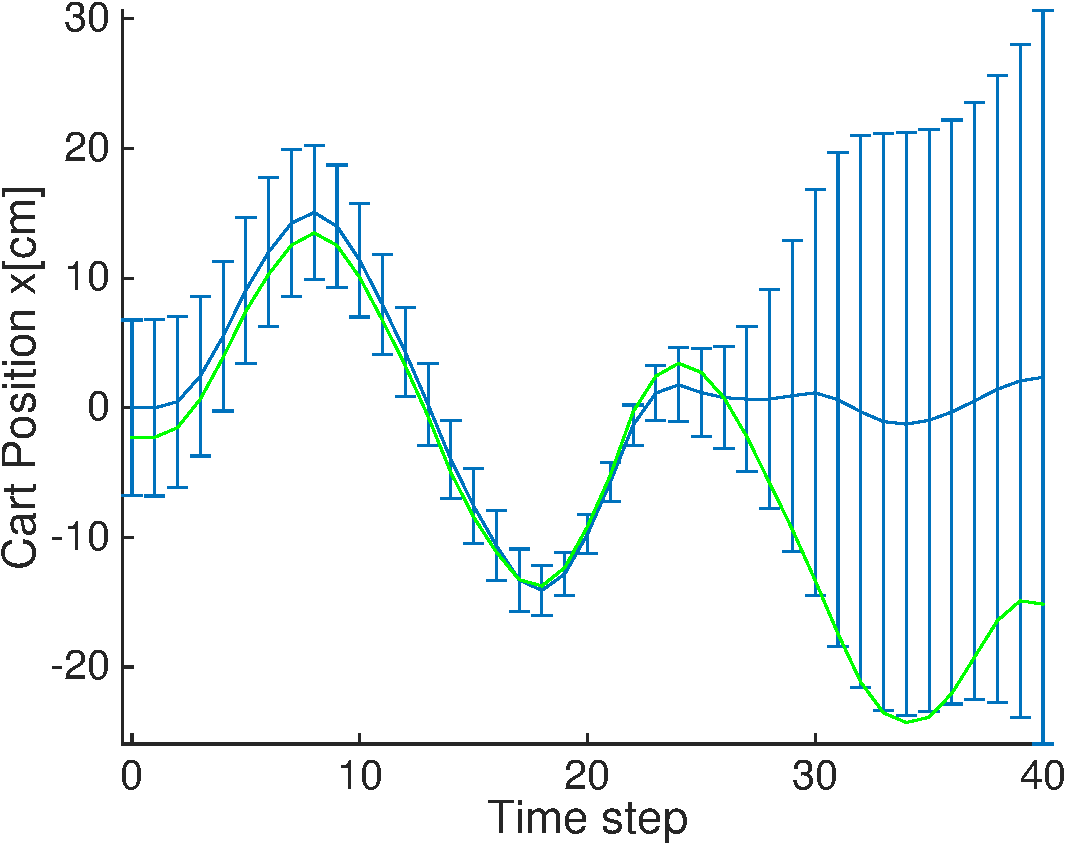
\includegraphics[width=60mm,scale=1]{plots/dmk3_pred_x}}{\caption{The predicted trajectory of $x$.}\label{fig:exps:double:3predx}}
    \end{floatrow}
    \begin{floatrow}
    \ffigbox[\FBwidth][\FBheight][t]{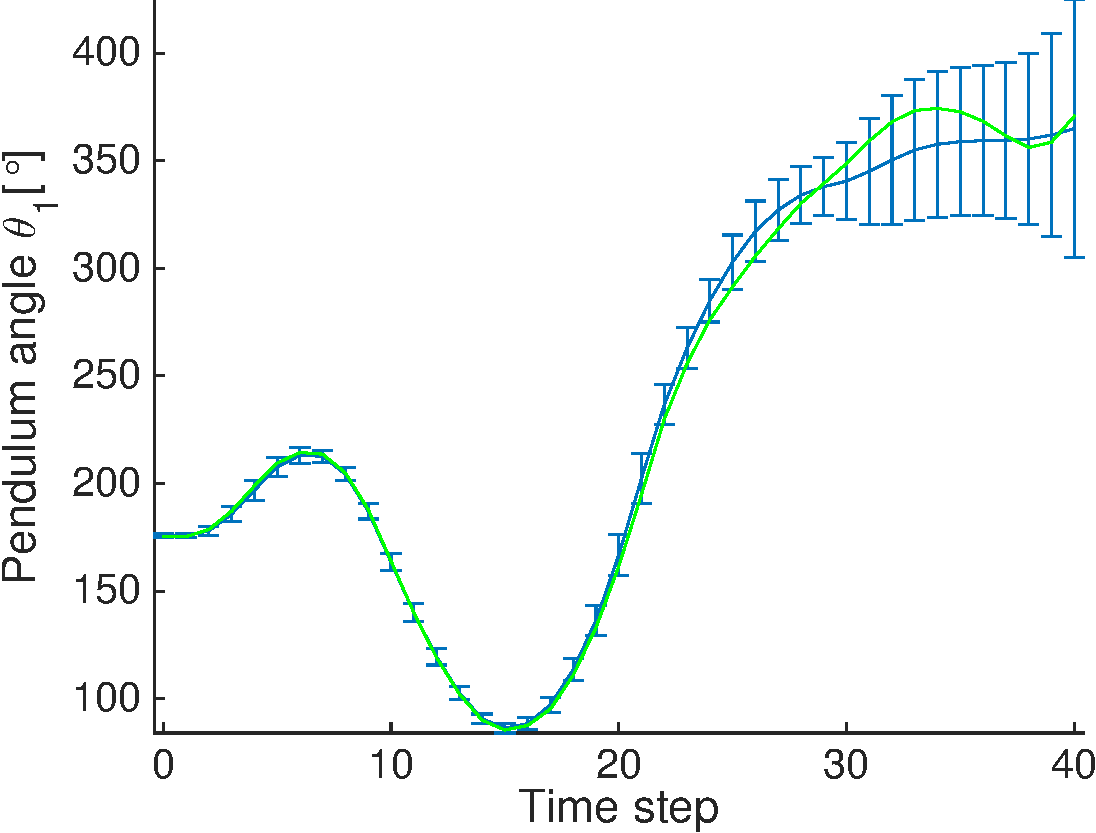
\includegraphics[width=60mm,scale=1]{plots/dmk3_pred_theta1}}{\caption{The predicted trajectory of $\theta_{1}$.}\label{fig:exps:double:3predtheta1}}
    \ffigbox[\FBwidth][\FBheight][t]{\includegraphics[width=60mm,scale=1]{plots/dmk3_pred_theta2}}{\caption{The predicted trajectory of $\theta_{2}$.}\label{fig:exps:double:3predtheta2}}
    \end{floatrow}
    \begin{floatrow}
    \ffigbox[\FBwidth][\FBheight][t]{\includegraphics[width=60mm,scale=1]{plots/dmk3_pred_u}}{\caption{The predicted action applied to the pendulum.}\label{fig:exps:double:3predu}}
    \end{floatrow}
\end{figure}